\documentclass[conference]{IEEEtran}
\IEEEoverridecommandlockouts
\usepackage{cite}
\usepackage{amsmath,amssymb}
\usepackage{graphicx}
\usepackage{booktabs}
\usepackage{xcolor}
\usepackage{url}
\usepackage[hidelinks]{hyperref}

% Notas de rascunho (remover antes da submissao)
\newcommand{\todo}[1]{\textcolor{red}{[TODO: #1]}}

\begin{document}

\title{Compression Hides Open-World Failures:\\INT8 Quantization and Unknown-Species Detection\\in Embedded Forest Species Recognition\\
\thanks{This work was supported by the National Council for Scientific and Technological Development (CNPq), Brazil, grants 401484/2025-4 and 303298/2022-7.}}

\author{\IEEEauthorblockN{Luiz S. Oliveira}
\IEEEauthorblockA{Department of Informatics\\
Federal University of Paran\'a (UFPR)\\
Curitiba, Brazil\\
lesoliveira@inf.ufpr.br}
\and
\IEEEauthorblockN{\todo{co-author}}
\IEEEauthorblockA{\todo{affiliation}}}

\maketitle

\begin{abstract}
Forest species recognition in the field requires models that run on smartphones or single-board computers and that can flag species they were not trained on, since no model covers all commercial timbers. INT8 quantization is the standard way to fit these models on ARM devices, and it is usually validated by closed-set accuracy alone. We show that this practice can hide a large loss in open-world reliability. Using a macroscopic (41 species) and a microscopic (112 species) wood image dataset, four backbones (MobileNetV3-Large, MobileNetV2, EfficientNet-Lite0 and ResNet-18), five post-hoc unknown detectors and ten random known/unknown species splits, we compare full-precision models with their INT8 versions under the default PyTorch configuration for ARM (QNNPACK). For the three depthwise-separable backbones, post-training quantization increases the rate of unknown species accepted as known (FPR at 95\% TPR) by 2 to 29 percentage points, consistently across splits, while closed-set accuracy often changes by less than one point. ResNet-18 is unaffected. Ablations trace the problem to per-tensor weight quantization, the backend default, which alone reproduces most of the degradation. The size of the effect follows the weight quantization error in the depthwise layers. Quantizing weights per channel restores accuracy and brings the increase to at most 2.2 points, at a cost of 0.2 to 0.4\,MB and no measurable CPU latency. Quantization-aware training brings no further gain. Compressed open-world models must therefore be validated with open-set metrics, and we recommend per-channel weight quantization combined with feature-based detectors for field deployment.
\end{abstract}

\begin{IEEEkeywords}
open-set recognition, out-of-distribution detection, quantization, edge devices, forest species recognition
\end{IEEEkeywords}

\section{Introduction}

Identifying the species of a piece of wood is a routine task in timber trade inspection and in the enforcement of environmental law. It usually requires a trained wood anatomist or a laboratory. Image-based recognition has reached very high closed-set accuracy on both macroscopic and microscopic wood images~\cite{martins2013database,paula2014forest,hafemann2014forest,ravindran2018meliaceae}, which makes a portable tool attractive: an inspector takes a picture with a phone or a single-board computer and obtains the species on the spot, without connectivity.

Two requirements follow from this scenario. The first is that the model must work in an open world. Thousands of species are traded, no training set covers all of them, and a closed-set classifier always answers with one of the species it knows. For an inspector, an unknown protected species classified with confidence as a common one is the worst possible error. The model must therefore score how familiar an input is and reject inputs from unknown species~\cite{scheirer2013open,bendale2015open,vaze2022open}. The second requirement is that the model must run on the device. INT8 quantization is the standard way to achieve this: it reduces the model about four times and speeds up inference several times on ARM CPUs~\cite{jacob2018quantization,krishnamoorthi2018quantizing}.

Quantized models are almost always validated by their closed-set accuracy. This raises the question addressed in this paper: \emph{does a quantized model that preserves accuracy also preserve its ability to recognize what it does not know?} Recent studies on large vision-language models and vision transformers report that quantization affects out-of-distribution (OOD) detection, sometimes for the better, and that the effect largely follows the change in accuracy~\cite{bouguerra2025less,kuang2026vit}. Much less is known about the compact convolutional networks that are actually deployed on phones and single-board computers.

We answer this question with a controlled study on two wood datasets and four backbones. Our contributions are:
\begin{itemize}
\item We show that INT8 post-training quantization with the default PyTorch configuration for ARM (QNNPACK) degrades unknown-species detection in all three depthwise-separable backbones, by up to 7.4 percentage points (pp) of FPR@95 for MobileNetV3 and up to 28.7\,pp for EfficientNet-Lite0, consistently across ten splits, while closed-set accuracy often changes by less than one point.
\item Through ablations, we trace the problem to per-tensor weight quantization in depthwise layers, and we show that the magnitude of the effect follows the weight quantization error of these layers.
\item We describe how the failure happens: quantization lowers the scores of known images more than those of unknown ones, which lowers the acceptance threshold and lets unknown species in.
\item We show that per-channel weight quantization removes most of the degradation at negligible cost, that quantization-aware training (QAT) adds nothing beyond it, and that feature-based detectors are the most robust choice.
\end{itemize}
Code, splits and all per-seed results are publicly available.\footnote{\url{https://github.com/lesoliveira/woodCompressao}}

\section{Related Work}

\textbf{Forest species recognition.} Public datasets of macroscopic~\cite{paula2014forest} and microscopic~\cite{martins2013database} wood images have supported a long line of work, from texture descriptors to deep networks~\cite{hafemann2014forest}. Field-oriented systems based on CNNs have also been proposed for species of commercial and conservation interest~\cite{ravindran2018meliaceae}. These works evaluate closed-set accuracy of full-precision models.

\textbf{Open-set and OOD detection.} Open-set recognition asks a classifier to reject inputs from classes not seen in training~\cite{scheirer2013open,bendale2015open}. A strong closed-set classifier combined with a post-hoc score is a competitive baseline~\cite{vaze2022open}. Post-hoc scores can be computed from the logits, as the maximum softmax probability (MSP)~\cite{hendrycks2017baseline}, the maximum logit~\cite{hendrycks2022scaling} and the energy~\cite{liu2020energy}, or from intermediate features, as the Mahalanobis distance~\cite{lee2018simple} and the distance to the $k$-th nearest training sample~\cite{sun2022knn}. We use these five scores because they require no retraining and can run on the device.

\textbf{Quantization and its side effects.} Integer-only inference~\cite{jacob2018quantization} is the basis of the quantization tools of the main frameworks. Weights can share a single scale per tensor or have one scale per output channel. Per-tensor weight quantization is known to hurt the accuracy of MobileNets, because the ranges of depthwise filters differ widely~\cite{krishnamoorthi2018quantizing,nagel2019dfq,nagel2021white}. Compression can also change model behavior in ways that the average accuracy does not reveal~\cite{hooker2019forget}, and it can either hurt or improve OOD robustness~\cite{diffenderfer2021winning}. For OOD detection specifically, quantization of CLIP-like models was found to be often harmless or even beneficial, with OOD performance strongly coupled to accuracy~\cite{bouguerra2025less}, while low-bit vision transformers lose OOD detection performance~\cite{kuang2026vit}. Our study differs in three ways: it targets the compact CNNs used on edge devices, it shows a case where open-set reliability degrades \emph{without} a matching loss of accuracy, and it identifies a concrete cause and fix in the default quantization configuration.

\section{Experimental Protocol}

\subsection{Datasets}

The \emph{macroscopic} dataset~\cite{paula2014forest} has 2,942 images of 41 species, acquired at $3264\times 2448$ pixels, with 37 to 99 images per species. The \emph{microscopic} dataset~\cite{martins2013database} has 2,240 images of 112 species (37 softwoods and 75 hardwoods), 20 images per species, at $1024\times 768$ pixels. Both were acquired in the laboratory.

A phase-correlation check between all pairs of images of the same species found exact duplicates (10 pairs) and overlapping fields of view in the microscopic dataset, and overlapping photographs of the same surface in the macroscopic dataset. For the microscopic dataset, overlapping images are grouped and always assigned to the same partition. For the macroscopic dataset we kept the per-image split and verified that removing the test images that overlap a training image changes no conclusion (Section~\ref{sec:extra}).

\subsection{Open-set protocol}

For each of ten random seeds, half of the species are drawn as \emph{known} (20 of 41 and 56 of 112) and the others as \emph{unknown}. Images of known species are split into training, validation and test sets (60/20/20). Unknown species appear only at test time. Each test set has about 290 known and 1,500 unknown images (macro) or 220 known and 1,120 unknown images (micro). All comparisons between a model and its quantized version are paired: same seed, same split and same test images.

\subsection{Models and training}

We use MobileNetV3-Large~\cite{howard2019searching}, MobileNetV2~\cite{sandler2018mobilenetv2}, EfficientNet-Lite0~\cite{tan2019efficientnet} and ResNet-18~\cite{he2016deep}, all pretrained on ImageNet. The first three are built from depthwise-separable convolutions and are typical edge models. ResNet-18 uses only standard convolutions. Images are resized to a shorter side of 672 (macro) or 768 (micro) pixels. Training uses random $224\times 224$ crops and SGD for 15 epochs, keeping the epoch with the best validation accuracy. At test time an image is represented by a grid of 12 non-overlapping patches, and logits and features are averaged over the patches.

We use the quantizable versions of the torchvision models and the timm~\cite{wightman2019timm} implementation of EfficientNet-Lite0. As in torchvision's quantizable MobileNetV2, ReLU6 is replaced by ReLU in EfficientNet-Lite0 before fine-tuning, because the QNNPACK backend cannot fuse ReLU6 with the convolution. The FP32 and INT8 models therefore share the same architecture.

\subsection{Quantization}

All models are quantized with PyTorch~\cite{paszke2019pytorch} (eager mode for the torchvision models, FX mode for EfficientNet-Lite0) and run with real INT8 kernels of the QNNPACK backend, which PyTorch uses on ARM CPUs such as those of phones, Raspberry Pi boards and Apple M chips. The \emph{default} post-training quantization (PTQ) uses the default QNNPACK configuration: symmetric INT8 weights with \emph{one scale per tensor} and activations calibrated with a histogram observer on 100 training images. The \emph{per-channel} variant changes only the weights, which receive one scale per output channel. QAT starts from the FP32 model and fine-tunes it for three epochs (learning rate $10^{-4}$) with fake quantization. To separate the effect of quantization from that of extra fine-tuning, each QAT model is compared with a \emph{control} that receives exactly the same fine-tuning without quantization.

\subsection{Unknown detection and metrics}

We use five post-hoc scores: MSP~\cite{hendrycks2017baseline}, MaxLogit~\cite{hendrycks2022scaling} and Energy~\cite{liu2020energy} (logit-based), and kNN ($k=5$, cosine)~\cite{sun2022knn} and Mahalanobis with a shared Ledoit-Wolf covariance~\cite{lee2018simple,ledoit2004well} on the penultimate features (feature-based). Feature-based detectors are fit on the training features of the model being evaluated, FP32 or INT8.

We report closed-set accuracy on known species and FPR@95, the fraction of unknown images accepted when the threshold accepts 95\% of the known ones. FPR@95 is the operational quantity of interest: the rate of unknown species that would be accepted as known. Differences between a model and its reference are computed per seed, and their significance is assessed with a paired Wilcoxon signed-rank test~\cite{wilcoxon1945individual} over the ten seeds. Latency is the median time per image (12 patches) with four threads on an Apple M CPU.

\section{Results}

\subsection{Default INT8 quantization degrades unknown detection}

\begin{table*}[t]
\centering
\caption{Closed-set accuracy and unknown-species detection (FPR@95, \%) of the FP32 models, and paired differences (percentage points, mean over 10 seeds) caused by INT8 post-training quantization with per-tensor weights (the PyTorch QNNPACK default) and with per-channel weights. Positive $\Delta$FPR@95 means more unknown species accepted as known. Paired Wilcoxon test: $^{\dagger}p<0.05$, $^{\ddagger}p<0.01$.}
\label{tab:main}
\setlength{\tabcolsep}{3.2pt}
\footnotesize
\begin{tabular}{ll ccc c cccc c cccc}
\toprule
 & & \multicolumn{3}{c}{FP32} & & \multicolumn{4}{c}{INT8, per-tensor weights (default)} & & \multicolumn{4}{c}{INT8, per-channel weights} \\
\cmidrule(lr){3-5}\cmidrule(lr){7-10}\cmidrule(lr){12-15}
Data & Backbone & Acc. & \multicolumn{2}{c}{FPR@95} & & $\Delta$Acc. & \multicolumn{2}{c}{$\Delta$FPR@95} & MB & & $\Delta$Acc. & \multicolumn{2}{c}{$\Delta$FPR@95} & MB \\
 & & & Energy & kNN & & & Energy & kNN & & & & Energy & kNN & \\
\midrule
Macro & MobileNetV3-L & 99.2 & 12.7 & 7.9 &  & -0.79$^{\dagger}$ & +7.4$^{\ddagger}$ & +2.8$^{\ddagger}$ & 4.2 &  & +0.04 & +2.0$^{\ddagger}$ & +0.1 & 4.5 \\
 & MobileNetV2 & 99.4 & 20.2 & 8.0 &  & -0.14 & +2.2$^{\dagger}$ & +0.0 & 2.3 &  & -0.10 & -0.3 & +0.2 & 2.5 \\
 & EfficientNet-Lite0 & 99.2 & 13.6 & 11.5 &  & -7.52$^{\dagger}$ & +28.7$^{\ddagger}$ & +12.0$^{\dagger}$ & 3.3 &  & +0.04 & +1.2$^{\dagger}$ & +0.2 & 3.7 \\
 & ResNet-18 & 99.3 & 15.2 & 8.4 &  & -0.10 & +0.8 & +0.0 & 10.7 &  & +0.00 & -0.1 & +0.1 & 10.8 \\
\midrule
Micro & MobileNetV3-L & 99.1 & 8.8 & 26.6 &  & -0.32 & +7.4$^{\ddagger}$ & +4.8$^{\ddagger}$ & 4.2 &  & +0.09 & +1.3$^{\ddagger}$ & -0.5 & 4.5 \\
 & MobileNetV2 & 99.2 & 8.4 & 14.5 &  & -0.18 & +2.8$^{\ddagger}$ & +2.2$^{\dagger}$ & 2.3 &  & -0.09 & -0.2 & +0.5 & 2.6 \\
 & EfficientNet-Lite0 & 98.8 & 11.0 & 29.7 &  & -0.72 & +12.1$^{\ddagger}$ & +6.4$^{\dagger}$ & 3.4 &  & -0.27 & +0.8 & -0.6 & 3.7 \\
 & ResNet-18 & 98.9 & 9.7 & 21.7 &  & -0.09 & -0.1 & -0.4 & 10.7 &  & -0.04 & +0.2 & -0.3 & 10.8 \\
\bottomrule
\end{tabular}
\end{table*}

Table~\ref{tab:main} and Fig.~\ref{fig:deltas} summarize the main result. With the default configuration, quantization increases FPR@95 in the three depthwise-separable backbones on both datasets. For MobileNetV3, the Energy detector accepts 7.4\,pp more unknown images on each dataset, which means 58\% more on the macroscopic dataset (12.7\% to 20.2\%), and the increase occurs in 10 of 10 seeds. MobileNetV2 is less affected (2.2 and 2.8\,pp). EfficientNet-Lite0 is the most affected: 28.7\,pp on the macroscopic and 12.1\,pp on the microscopic dataset. ResNet-18 shows no significant change.

\begin{figure*}[t]
\centering
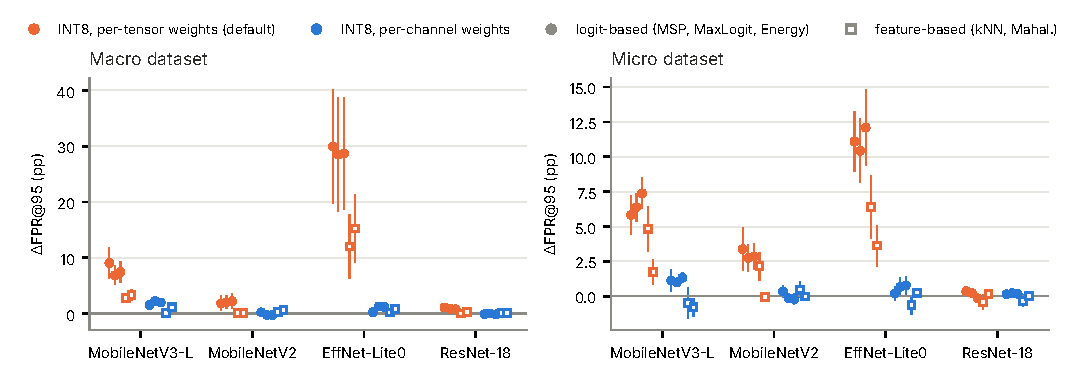
\includegraphics[width=\textwidth]{figs/deltas.pdf}
\caption{Paired $\Delta$FPR@95 of INT8 PTQ against FP32 for each backbone and detector (mean $\pm$ standard error over 10 seeds). Circles: logit-based detectors (MSP, MaxLogit, Energy). Squares: feature-based detectors (kNN, Mahalanobis). Per-channel weights (blue) remove most of the degradation caused by the default per-tensor weights (orange).}
\label{fig:deltas}
\end{figure*}

These losses are often invisible to closed-set accuracy. MobileNetV3 loses 0.79\,pp of accuracy on the macroscopic dataset and 0.32\,pp (not significant) on the microscopic one. The clearest case is EfficientNet-Lite0 on the microscopic dataset: accuracy drops by 0.72\,pp (not significant, $p=0.06$) while the rate of accepted unknown species doubles, from 11.0\% to 23.1\%. A model validated by accuracy alone would be approved. On the macroscopic dataset the same backbone also loses 7.5\,pp of accuracy, but FPR@95 grows from 13.6\% to 42.3\%, so the damage to unknown detection is much larger than the damage to classification.

Logit-based detectors suffer the most. Feature-based detectors also degrade under default PTQ, by up to 12.0\,pp for kNN, but always less than Energy in the depthwise backbones.

\subsection{The cause is per-tensor weight quantization}

\begin{table}[t]
\centering
\caption{PTQ ablation on MobileNetV3-L: paired differences to FP32 (pp, 10 seeds). \emph{Weights only}: weights quantized to INT8, activations kept in FP32.}
\label{tab:ablation}
\setlength{\tabcolsep}{2.6pt}
\footnotesize
\resizebox{\columnwidth}{!}{%
\begin{tabular}{l ccc ccc}
\toprule
 & \multicolumn{3}{c}{Macro} & \multicolumn{3}{c}{Micro} \\
\cmidrule(lr){2-4}\cmidrule(lr){5-7}
PTQ configuration & $\Delta$Acc. & \multicolumn{2}{c}{$\Delta$FPR@95} & $\Delta$Acc. & \multicolumn{2}{c}{$\Delta$FPR@95} \\
 & & Energy & kNN & & Energy & kNN \\
\midrule
Default (per-tensor weights) & -0.79$^{\dagger}$ & +7.4$^{\ddagger}$ & +2.8$^{\ddagger}$ & -0.32 & +7.4$^{\ddagger}$ & +4.8$^{\ddagger}$ \\
Per-channel weights & +0.04 & +2.0$^{\ddagger}$ & +0.1 & +0.09 & +1.3$^{\ddagger}$ & -0.5 \\
Weights only, per-tensor & -0.60$^{\ddagger}$ & +5.9$^{\ddagger}$ & +3.2$^{\ddagger}$ & -0.18 & +5.4$^{\ddagger}$ & +3.7$^{\dagger}$ \\
Weights only, per-channel & +0.11 & +0.3 & -0.4 & +0.05 & +0.7$^{\dagger}$ & +0.9 \\
Last linear layer in FP32 & -0.83$^{\dagger}$ & +7.4$^{\ddagger}$ & +2.8$^{\ddagger}$ & -0.32 & +7.3$^{\ddagger}$ & +4.8$^{\ddagger}$ \\
Last 3 blocks + classifier in FP32 & -0.68$^{\dagger}$ & +7.2$^{\ddagger}$ & +2.6$^{\ddagger}$ & -0.27 & +6.9$^{\ddagger}$ & +5.3$^{\ddagger}$ \\
Calibration with 25 images & -0.50$^{\dagger}$ & +6.9$^{\ddagger}$ & +3.1$^{\dagger}$ & -0.41 & +9.2$^{\ddagger}$ & +4.1$^{\dagger}$ \\
Calibration with 400 images & -0.62$^{\dagger}$ & +7.1$^{\ddagger}$ & +2.9$^{\ddagger}$ & -0.09 & +7.2$^{\ddagger}$ & +4.1$^{\dagger}$ \\
MinMax activation observer & -2.78$^{\ddagger}$ & +39.8$^{\ddagger}$ & +8.6$^{\ddagger}$ & -10.99$^{\ddagger}$ & +28.3$^{\ddagger}$ & +16.4$^{\ddagger}$ \\
\bottomrule
\end{tabular}}
\end{table}

Table~\ref{tab:ablation} isolates the cause for MobileNetV3. Quantizing \emph{only the weights} per tensor, with activations kept in FP32, reproduces most of the effect (5.9 of 7.4\,pp on the macroscopic and 5.4 of 7.4\,pp on the microscopic dataset). Quantizing only the weights per channel reproduces almost nothing. Keeping the last linear layer, or the last three blocks and the classifier, in FP32 does not help, and neither does a smaller or a larger calibration set. The problem is not located at the end of the network: the relative quantization error of the activations grows block by block, and at the logits it reaches 26\% for known and 34\% for unknown images (macro). Finally, the choice of activation observer matters: a MinMax observer is catastrophic (up to 39.8\,pp of FPR@95 and 11\,pp of accuracy), which shows how fragile these models are to the quantization configuration.

\subsection{Why some architectures suffer more}

\begin{table}[t]
\centering
\caption{INT8 weight quantization error (BN folded), mean over layers, checkpoints and datasets. Spread: largest over median per-channel weight range. Dead: channels (non-zero in FP32) whose weights all round to zero with a per-tensor scale. Last column: $\Delta$FPR@95 (Energy) of default PTQ, macro/micro.}
\label{tab:weights}
\setlength{\tabcolsep}{2.6pt}
\footnotesize
\begin{tabular}{l cccc c c}
\toprule
 & \multicolumn{4}{c}{Depthwise layers} & All & \\
\cmidrule(lr){2-5}\cmidrule(lr){6-6}
Backbone & Spread & Err.\ PT & Err.\ PC & Dead & Err.\ PT & $\Delta$FPR@95 \\
\midrule
MobileNetV3-L & 4.6$\times$ & 2.0\% & 0.6\% & 0.1\% & 2.3\% & +7.4/+7.4 \\
MobileNetV2 & 4.3$\times$ & 1.8\% & 0.4\% & 0.9\% & 1.5\% & +2.2/+2.8 \\
EfficientNet-Lite0 & 5.8$\times$ & 3.3\% & 0.6\% & 2.8\% & 2.6\% & +28.7/+12.1 \\
ResNet-18 & -- & -- & -- & -- & 3.4\% & +0.8/-0.1 \\
\bottomrule
\end{tabular}
\end{table}

With a per-tensor scale, all channels of a layer share the step size dictated by the channel with the largest weights. Channels with small weights keep few quantization levels, or round entirely to zero. Table~\ref{tab:weights} measures this on the FP32 checkpoints, after folding batch normalization into the convolutions as done by the quantizer. The overall weight error does not explain the results: ResNet-18 has the largest error over all layers (3.4\%) and no degradation. In a standard convolution, each output sums contributions from hundreds of input channels and rounding errors tend to cancel. In a depthwise convolution, each output depends on a single filter and its error propagates directly. Among the depthwise backbones, the weight error of the depthwise layers follows the degradation (Spearman $\rho=0.89$ over the six dataset-backbone pairs). EfficientNet-Lite0 has the most uneven filters, with some late layers where the largest channel range is 63 times the median and 15\% of the channels are zeroed. Per-channel scales reduce the depthwise weight error 3 to 5.5 times in every backbone.

The weight error does not explain everything. MobileNetV3 and MobileNetV2 have similar depthwise weight errors (2.0\% and 1.8\%), but MobileNetV3 degrades three times more, which suggests that it amplifies the same error more. With four backbones, these correlations are indicative rather than conclusive.

\subsection{How the failure happens}

\begin{figure*}[t]
\centering
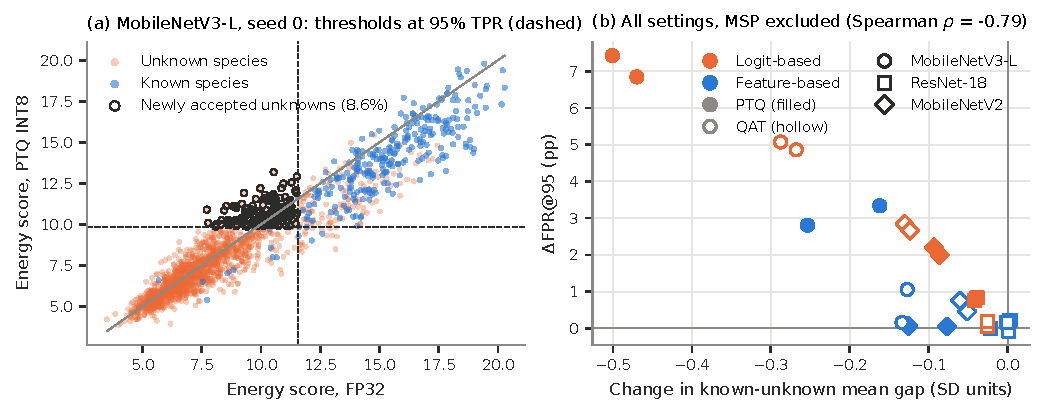
\includegraphics[width=\textwidth]{figs/mechanism_macro.pdf}
\caption{(a) Energy score of each test image for the FP32 and the PTQ INT8 MobileNetV3 (macroscopic dataset, one seed). Dashed lines: thresholds at 95\% TPR. Known images (blue) fall below the diagonal, unknown images (orange) stay on it, and the threshold moves down. (b) Change in the mean gap between known and unknown scores (in units of the reference standard deviation) against $\Delta$FPR@95, for MobileNetV3, MobileNetV2 and ResNet-18, PTQ and QAT, and all detectors except MSP, whose score saturates (macroscopic dataset).}
\label{fig:mechanism}
\end{figure*}

Quantization does not add noise uniformly. For MobileNetV3 with the Energy score, it lowers the scores of known images by 0.67 standard deviations on average and those of unknown images by only 0.17 (macro). On the microscopic dataset the values are 0.78 and 0.20. The threshold that accepts 95\% of the known images moves down with them, and unknown images just below the old threshold are now accepted (Fig.~\ref{fig:mechanism}a). The exchange is very asymmetric: 8.5\% of the unknown images become accepted and only 1.1\% become rejected. Across backbones, comparisons and detectors, the loss of separation between known and unknown scores predicts the increase in FPR@95 (Spearman $\rho=-0.79$, Fig.~\ref{fig:mechanism}b). Confident inputs, which produce the largest activations, appear to be the most distorted by coarse weights, and feature-based scores lose less separation than logit-based ones.

\subsection{Per-channel weights and QAT}

\begin{table}[t]
\centering
\caption{QAT against a control with the same fine-tuning and no quantization: paired $\Delta$FPR@95 (pp, 10 seeds). Accuracy changed by at most 0.11\,pp in all cases.}
\label{tab:qat}
\setlength{\tabcolsep}{3pt}
\footnotesize
\begin{tabular}{ll cc cc}
\toprule
 & & \multicolumn{2}{c}{QAT, per-tensor} & \multicolumn{2}{c}{QAT, per-channel} \\
\cmidrule(lr){3-4}\cmidrule(lr){5-6}
Data & Backbone & Energy & kNN & Energy & kNN \\
\midrule
Macro & MobileNetV3-L & +5.1$^{\ddagger}$ & +0.2 & +2.7$^{\ddagger}$ & -0.2 \\
 & MobileNetV2 & +2.8 & +0.8 & +1.1 & -0.2 \\
\midrule
Micro & MobileNetV3-L & -0.5 & +1.5 & -2.3 & +0.3 \\
 & MobileNetV2 & +2.1 & +3.7 & +0.4 & -0.3 \\
\bottomrule
\end{tabular}
\end{table}

Per-channel weights remove most of the degradation in every depthwise backbone (Table~\ref{tab:main}, Fig.~\ref{fig:deltas}). Accuracy returns to the FP32 level, the increase in FPR@95 falls to at most 2.2\,pp for logit-based detectors and to at most 1.1\,pp for feature-based ones, with kNN never significant. The cost is small: 0.2 to 0.4\,MB more per model and no measurable difference in latency (for example, 20 against 21\,ms per image for MobileNetV3, against 107\,ms in FP32, and 28\,ms for both EfficientNet-Lite0 variants, against 219\,ms in FP32).

QAT does not improve on per-channel PTQ (Table~\ref{tab:qat}). With per-tensor weights, QAT still increases FPR@95 of MobileNetV3 by 5.1\,pp on the macroscopic dataset in 10 of 10 seeds, although its accuracy equals that of the control (difference below 0.1\,pp). With per-channel weights, the increase falls to 2.7\,pp, similar to per-channel PTQ (2.0\,pp), and vanishes in the other settings. Since PTQ requires no retraining, per-channel PTQ is the practical choice.

\subsection{Additional analyses}
\label{sec:extra}

\textbf{Near and far unknowns.} On the microscopic dataset, unknown species whose genus is among the known species are harder even in FP32 (FPR@95 of 12.0\% against 7.6\% for the other genera, MobileNetV3, Energy). Default PTQ hurts them slightly more (+8.8 against +6.9\,pp), and the same holds for softwoods against hardwoods (+8.7 against +6.8\,pp).

\textbf{Overlapping images.} Removing from the macroscopic test sets the images that overlap a training image (about 11 per seed) changes the MobileNetV3 result from +7.4 to +7.6\,pp for PTQ and from +5.1 to +5.4\,pp for QAT, with the same significance.

\textbf{Latency of ResNet-18.} On the Apple M CPU, the INT8 ResNet-18 is slower than its FP32 version (101 against 67\,ms), because QNNPACK targets mobile architectures. This confirms that ResNet-18 is not a realistic edge model, but its robustness serves as a reference.

\section{Discussion and Limitations}

Our results show that closed-set accuracy is not a sufficient criterion to validate a quantized open-world model. A deployment pipeline that checks accuracy would accept models that admit up to twice as many unknown species. The default configuration matters: per-tensor weights are the default of the PyTorch QNNPACK backend, and some accelerators do not support per-channel weights at all, so the problem cannot always be avoided by configuration. In such cases, open-set metrics should be part of the acceptance tests, and feature-based detectors are the safer choice.

The study has limitations. The datasets were acquired in the laboratory, and field images may behave differently. Latency was measured on an Apple M CPU, which uses the same backend as phones and Raspberry Pi boards and gives the same predictions, but absolute times on these devices will be higher. \todo{Raspberry Pi 5 measurements, if available.} Replacing ReLU6 with ReLU in EfficientNet-Lite0 removes the bounded activation for which the original model was designed, which may contribute to its large per-tensor degradation. We studied only 8-bit uniform quantization. Lower bit widths and pruning remain to be evaluated.

\section{Conclusion}

INT8 quantization with per-tensor weights, the default PyTorch configuration for ARM, increases the rate of unknown wood species accepted as known by up to 7.4\,pp in MobileNetV3 and 28.7\,pp in EfficientNet-Lite0, while closed-set accuracy often changes by less than one point. The cause is the coarse quantization of depthwise filters. Quantizing weights per channel and using a feature-based detector restores open-world reliability at negligible cost. For field tools that must say ``I do not know this species'', we recommend validating compressed models with open-set metrics as a matter of course.

\bibliographystyle{IEEEtran}
\bibliography{refs}

\end{document}
